%
\section{Results and Discussion}

\begin{table*}[h]
  \setlength{\tabcolsep}{3pt}
  \caption{Performance of, and parameters for the Shape Matching Element Method on all examples. All wall-clock timings are reported in seconds, physical parameters are
  reported with appropriate units. $\rho$ is the applied density, \textbf{E} is the  Young's Modulus and \revise{$\nu$} is the Poisson's ratio.
  \textbf{Sample} is the time taken to sample and construct $\samp{\Jnurbs}$ and $\samp{\Pmatx}$, \textbf{Quad} is the time taken to generate quadrature points via raycasting,
  \textbf{Weights} is the time to compute blending weights, \textbf{Build $\Pi$} is the time to build the projection operator, \textbf{Step} is the average time required to step the simulation (not including collision detection)
  \revise{and \textbf{Nnz} is the ratio of nonzeros to the total number of elements in the stiffness matrix. }
  \revise{We use linearly implicit time integration on all examples and thus the number of step per frame is 1 in the simulation.}
  }
  \label{tbl:perf}
  \begin{center}
  \begin{tabular}{l c c c c c c c c c c c}
   \textbf{Example} & $|\vc{q}|$ & \textbf{Material}&  $\rho$(kg/m$^3$) & \textbf{E}(Pa) & \revise{$\nu$} &\textbf{Sample}(s) & \textbf{Quad}(s)& \textbf{Weights}(s) & \textbf{Build $\Pi$}(s) & \textbf{Step}(s) & \revise{\textbf{Nnz}(\%)} \\
   \hline 
   \rowcolor[HTML]{DAE8FC}
   %\textbf{Cantilever (soft)}       & 564 & Jelly & $1 e^3$ & $1e^6$& 0.45 & $2.53 e^{-2}$ & $4.45 e^{-3}$ & $4.78 e^{-1}$ & $1.86 e^{-1}$ & $1.20 e^{0}$ \\
   %\textbf{Cantilever (stiff)}      & 564 & Rubber & $1 e^3$ & $5 e^6$ & 0.45 & $2.48 e^{-2}$ & $6.37 e^{-3}$ & $5.10 e^{-1}$ & $1.68 e^{-1}$ & $1.19 e^{0}$ \\
   \rowcolor[HTML]{DAE8FC} 
   \textbf{Rocket (soft)}           & 648 & Rubber & $1.27 e^3$ & $7 e^6$ & 0.40 & $2.83 e^{-2}$ & $5.62 e^{-3}$ & $5.58 e^{-1}$ & $6.83 e^{-2}$ & $1.26 e^{0}$ & \revise{100} \\
   \textbf{Rocket (stiff)}          & 648 & Steel & $8 e^3$ & $2 e^{11}$ & 0.32 & $2.56 e^{-2}$ & $5.97 e^{-3}$ & $4.59 e^{-1}$ & $3.48 e^{-2}$ & $9.99 e^{-2}$ & \revise{100} \\
   \rowcolor[HTML]{DAE8FC} 
   \textbf{Starship}                & 750 & Steel & $8 e^3$ & $2 e^{11}$ & 0.32 & $6.78 e^{-2}$ & $1.52 e^{-2}$ & $8.50 e^{-1}$ & $9.52 e^{-2}$ & $6.95 e^{-1}$ & \revise{100} \\
   \revise{\textbf{Beam (twist)}}   & \revise{756} & \revise{Rubber} & \revise{$1 e^3$} & \revise{$1 e^6$} & \revise{0.45} & \revise{$1.97 e^{-1}$} & \revise{$2.25 e^{-2}$} & \revise{$1.35 e^{0}$} & \revise{$5.16 e^{-1}$} & \revise{$3.95 e^{0}$} & \revise{46.94} \\
   \rowcolor[HTML]{DAE8FC} 
   \textbf{Lamppost}                & 942 & Rubber & $3 e^3$ & $1 e^6$ & 0.40 & $1.28 e^{-1}$ & $1.27 e^{-2}$ & $1.89 e^{0}$ & $1.07 e^{0}$ & $2.22 e^{0}$ & \revise{56.38} \\
   \textbf{Tire}                    & 1404 & Rubber/Steel & $2 e^3$/$3 e^3$ & $1 e^6$/$7 e^9$ & 0.47/0.35 & $1.74 e^{-1}$ & $1.32 e^{-2}$ & $1.82 e^{0}$ & $6.79 e^{-1}$ & $1.28 e^{1}$ & \revise{92.5} \\
   \rowcolor[HTML]{DAE8FC} 
   \textbf{Chicken}                 & 1773 & Jelly & $1.27 e^3$ & $1 e^4$ & 0.47 & $9.19 e^{-1}$ & $2.31 e^{-2}$ & $3.38 e^{0}$ & $1.91 e^{0}$ & $1.08 e^{1}$ & \revise{100} \\
   \textbf{Coffee mug (soft)}       & 1800 & Jelly & $1 e^3$ & $1 e^4$ & 0.47 & $4.18 e^{-1}$ & $2.87 e^{-2}$ & $3.77 e^{0}$ & $2.08 e^{0}$ & $1.19 e^{1}$ & \revise{100} \\ 
   \rowcolor[HTML]{DAE8FC} 
   \textbf{Coffee mug (stiff)}      & 1800 & Rubber & $1 e^3$ & $4 e^7$ & 0.40 & $4.15 e^{-2}$ & $1.17 e^{-2}$ & $6.86 e^{-1}$ & $1.09 e^{-1}$ & $5.00 e^{-1}$  & \revise{81.42} \\ 
   \textbf{Castle}                  & 1872 & Jelly & $1.27 e^3$ & $2 e^3$ & 0.45 & $4.84 e^{-1}$ & $1.44 e^{-2}$ & $1.52 e^{0}$ & $5.78 e^{-1}$ & $8.02 e^{0}$ & \revise{100} \\
   \rowcolor[HTML]{DAE8FC} 
   \textbf{Grumpy}                  & 2010 & Jelly & $1 e^3$ & $1 e^4$ & 0.40 & $2.92 e^{-1}$ & $1.23 e^{-2}$ & $2.29 e^{0}$ & $2.89 e^{0}$ & $6.02 e^{0}$ & \revise{84.15} \\    
   \textbf{Astronaut (soft)}        & 3609 & Rubber &  $1.27 e^3$  & $1 e^6$  & 0.47 & $2.47 e^{0}$ & $6.71 e^{-2}$ & $1.13 e^{1}$ & $1.09 e^{1}$ & $1.41 e^{1}$ & \revise{49.04} \\
   \rowcolor[HTML]{DAE8FC} 
   \revise{\textbf{Squid}}          & \revise{4347} & \revise{Jelly} & \revise{ $1 e^3$ } & \revise{$2 e^4$ } & \revise{0.40} & \revise{$4.48 e^{-1}$} & \revise{$2.47 e^{-2}$} & \revise{$1.54 e^{1}$} & \revise{$4.48 e^{1}$} & \revise{$6.73 e^{0}$} & \revise{25.47} \\
   \rowcolor[HTML]{DAE8FC} 
   \hline
  \end{tabular}
  \end{center}
  
  \end{table*}

% \begin{table*}[h]
%   \caption{Performance of, and parameters for the Shape Matching Element Method on all examples. All wall-clock timings are reported in seconds, physical parameters are
%   reported with appropriate units. $\rho$ is the applied density, \textbf{E} is the  Young's Modulus and $\mu$ is the Poisson's ratio.
%   \textbf{Sample} is the time taken to sample and construct $\samp{\Jnurbs}$ and $\samp{\Pmatx}$, \textbf{Quad} is the time taken to generate quadrature points via raycasting,
%   \textbf{Weights} is the time to compute blending weights, \textbf{Build $\Pi$} is the time to build the projection operator and  \textbf{Step} is the average time required to step the simulation (not including collision detection).
%   \revise{We use linearly implicit time integration on all examples and thus the number of step per frame is 1 in the simulation.}
%   }
%   \label{tbl:perf}
%   \begin{center}
%   \begin{tabular}{l c c c c c c c c c c}
%    \textbf{Example} & $|\vc{q}|$ & \textbf{Material}&  $\rho$(kg/m$^3$) & \textbf{E}(Pa) & $\mu$ &\textbf{Sample}(s) & \textbf{Quad}(s)& \textbf{Weights}(s) & \textbf{Build $\Pi$}(s)& \textbf{Step}(s) \\
%    \hline 
%    \rowcolor[HTML]{DAE8FC}
%    %\textbf{Cantilever (soft)}       & 564 & Jelly & $1 e^3$ & $1e^6$& 0.45 & $2.53 e^{-2}$ & $4.45 e^{-3}$ & $4.78 e^{-1}$ & $1.86 e^{-1}$ & $1.20 e^{0}$ \\
%    %\textbf{Cantilever (stiff)}      & 564 & Rubber & $1 e^3$ & $5 e^6$ & 0.45 & $2.48 e^{-2}$ & $6.37 e^{-3}$ & $5.10 e^{-1}$ & $1.68 e^{-1}$ & $1.19 e^{0}$ \\
%    \rowcolor[HTML]{DAE8FC} 
%    \textbf{Rocket (soft)}           & 648 & Rubber & $1.27 e^3$ & $7 e^6$ & 0.40 & $2.83 e^{-2}$ & $5.62 e^{-3}$ & $5.58 e^{-1}$ & $6.83 e^{-2}$ & $1.26 e^{0}$ \\
%    \textbf{Rocket (stiff)}          & 648 & Steel & $8 e^3$ & $2 e^{11}$ & 0.32 & $2.56 e^{-2}$ & $5.97 e^{-3}$ & $4.59 e^{-1}$ & $3.48 e^{-2}$ & $9.99 e^{-2}$ \\
%    \rowcolor[HTML]{DAE8FC} 
%    \textbf{Starship}                & 750 & Steel & $8 e^3$ & $2 e^{11}$ & 0.32 & $6.78 e^{-2}$ & $1.52 e^{-2}$ & $8.50 e^{-1}$ & $9.52 e^{-2}$ & $6.95 e^{-1}$ \\
%    \textbf{Lamppost}                & 942 & Rubber & $3 e^3$ & $1 e^6$ & 0.40 & $1.28 e^{-1}$ & $1.27 e^{-2}$ & $1.89 e^{0}$ & $1.07 e^{0}$ & $2.22 e^{0}$ \\
%    \rowcolor[HTML]{DAE8FC} 
%    \textbf{Tire}                    & 1404 & Rubber/Steel & $2 e^3$/$3 e^3$ & $1 e^6$/$7 e^9$ & 0.47/0.35 & $1.74 e^{-1}$ & $1.32 e^{-2}$ & $1.82 e^{0}$ & $6.79 e^{-1}$ & $1.28 e^{1}$ \\
%    \textbf{Chicken}                 & 1773 & Jelly & $1.27 e^3$ & $1 e^4$ & 0.47 & $9.19 e^{-1}$ & $2.31 e^{-2}$ & $3.38 e^{0}$ & $1.91 e^{0}$ & $1.08 e^{1}$ \\
%    \rowcolor[HTML]{DAE8FC} 
%    \textbf{Coffee mug (soft)}       & 1800 & Jelly & $1 e^3$ & $1 e^4$ & 0.47 & $4.18 e^{-1}$ & $2.87 e^{-2}$ & $3.77 e^{0}$ & $2.08 e^{0}$ & $1.19 e^{1}$  \\ 
%    \textbf{Coffee mug (stiff)}      & 1800 & Rubber & $1 e^3$ & $4 e^7$ & 0.40 & $4.15 e^{-2}$ & $1.17 e^{-2}$ & $6.86 e^{-1}$ & $1.09 e^{-1}$ & $5.00 e^{-1}$  \\ 
%    \rowcolor[HTML]{DAE8FC} 
%    \textbf{Castle}                  & 1872 & Jelly & $1.27 e^3$ & $2 e^3$ & 0.45 & $4.84 e^{-1}$ & $1.44 e^{-2}$ & $1.52 e^{0}$ & $5.78 e^{-1}$ & $8.02 e^{0}$ \\
%    \textbf{Grumpy}                  & 2010 & Jelly & $1 e^3$ & $1 e^4$ & 0.40 & $2.92 e^{-1}$ & $1.23 e^{-2}$ & $2.29 e^{0}$ & $2.89 e^{0}$ & $6.02 e^{0}$  \\    
%    \rowcolor[HTML]{DAE8FC} 
%    \textbf{Astronaut (soft)}        & 3609 & Rubber &  $1.27 e^3$  & $1 e^6$  & 0.47 & $2.47 e^{0}$ & $6.71 e^{-2}$ & $1.13 e^{1}$ & $1.09 e^{1}$ & $1.41 e^{1}$ \\
%    \textbf{Squid}                   & 4347 & Rubber &  $1 e^3$  & $2 e^4$  & 0.40 & $4.48 e^{-1}$ & $2.47 e^{-2}$ & $1.54 e^{1}$ & $4.48 e^{1}$ & $6.73 e^{0}$ \\
%    \rowcolor[HTML]{DAE8FC} 
%    \hline
%   \end{tabular}
%   \end{center}
  
%   \end{table*}

%\dave{we should show the nurbs model in rhino/fusion for every example, maybe an exploded view as well}

%\dave{mention that not so many standard NURBS models so we modelled lots of these ourselves .. show's power of approach that we can model and sim all these examples.}

%\dave{use as many different meshes as possible for figures (i.e try not to have the same mesh show up in more than one figure if possible).}

%\dave{we should report which models we made ourselves}
We implemented SEM using a combination of MATLAB and C++ using both GPToolbox~\cite{gptoolbox} and Bartels~\cite{bartels} for geometry processing and constitutive models 
respectively. Benchmarks were performed using a MacBook Pro with an Intel i5 2.3GHz processor, 16GB of RAM and an Intel Iris Plus Graphics 655 GPU.

\reftbl{perf} shows the size of all our examples along with performance statistics and relevant parameters. 
\revise{We also plot the sparsity patterns of several stiffness matrices in our examples in \reffig{stiffness_sparsity}. }
Note that the individual parts of all models are \emph{not connected}, and no continuity constraints or constructive solid geometry operations have been applied. 
Rather, the SEM approach implicitly couples the boundary parts together to allow for seamless volumetric simulation. 
We use quadratic deformation for all the animation results, except the rocket (stiff) and starship which use linear deformation.
Models were created using Autodesk Fusion 360 \cite{AutodeskFusion360} and \revise{Rhinoceros} 3D 7 \cite{mcneel-rhinoceros}. 
Please see the supplemental video for more animation results.
  
For raycasting operations and rendering we rely on Embree~\cite{10.1145/2601097.2601199} and Blender~\cite{blender}, and triangulate the NURBS surfaces, which only represents an implementation simplification. 
Our core algorithm is not dependent on triangulating the boundary, and an ideal alternative would be using a path tracer that directly accepts NURBS geometry.
For collision detection and handling, for simplicity we use the triangulation to detect inter-penetrations at each iteration, and attempt to move the collided vertex out of its collision surface using a spring-like penalty force, similar to \cite{10.1145/3355089.3356486, 10.1145/2010324.1964932}.
An ideal alternative would be adopting the implicit representation of the surfaces for collision detection and resolution \cite{10.1145/1516522.1516523, 10.1145/3306346.3323010}. 

\nicetohave{Would be nice to mention TNURBS, which would give us a good reason to include the wrench (which i really wanna do). I doubt we have time to do a 3 point bending test, but a simple elastic wrench simulation would be easy to cook up}
For handling trimmed NURBS surfaces, we augment our sampling of the surfaces by using raycasting integration in 2D. Trimmed NURBS may be defined by a boundary curve in the parametric space, so we raycast to find intersection intervals in the UV space on which quadrature points are generated. For rendering Trimmed NURBS, we discretize the the boundary curve as a polyline and use triangle \cite{shewchuk96b, SHEWCHUK200221} to form a boundary conforming triangulation. The vertices of this triangulation serve as fixed set of high resolution UV samples for constructing a render mesh.


%% Results that relate to preprocessing
% weights are good
% \begin{figure}
%   \centering
%   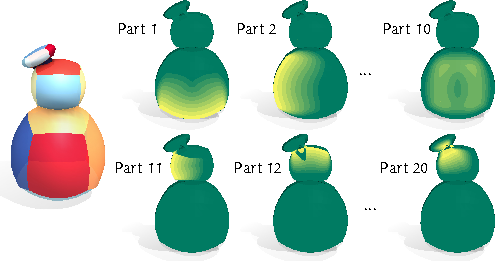
\includegraphics[width=3.33in]{figures/distance_weight_puft.pdf}
%   \caption{Our distance weights decay smoothly from 1.0 (yellow) to 0.0 (green) when moving away from its closest surface. Here we visualize the distribution of the distance weights (with cutoff distance 5.0) corresponding to each part.   
%   }
%   \label{fig:distance_weight_puft}
%   \vspace{-5pt}
% \end{figure} 
% %
% %
% \begin{figure}
%   \centering
%   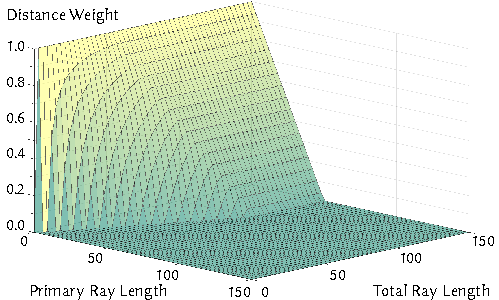
\includegraphics[width=3.33in]{figures/plot_distance_weight.pdf}
%   \caption{We plot the distance weight with respect to the primary and total ray length. Here the cutoff distance is 50.
%   }
%   \label{fig:plot_distance_weight}
%   \vspace{-5pt}
% \end{figure} 

%kinematic model is expressive
% \begin{figure}
%   \includegraphics[width=\columnwidth]{example-image-a}
%   \caption{Take an intesting geometry (maybe that geometry processing cacture), deform it, do our shape matching and then reconstruct the deformed pose. Do this for a bunch of poses (show's kinematic model is good).}
%   \label{fig:deform}
% \end{figure}

%% Results that relate to simulation output
%correctness
\begin{figure}[h]
  \includegraphics[width=\columnwidth]{figures/patch_test.pdf}
  \caption{2D patch test. By applying affine transformations to the boundary of the original undeformed model (left), we show that solving the static problem gives rigid motion for rotation and constant strain for shearing and stretching (right).}
  % \caption{2D patch test. Left: the original undeformed model defined by four surface elements on the boundary. Right:  applying affine transformations to the boundary and show that solving the static problem gives rigid motion for rotation and constant strain for shearing and stretching}
  \label{fig:patchtest}
\end{figure}

\begin{figure}[h]
  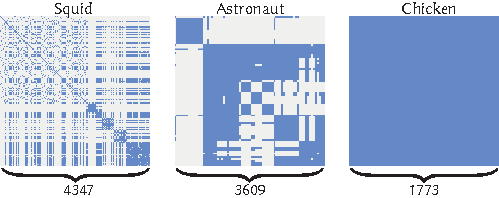
\includegraphics[width=\columnwidth]{figures/stiffness_sparsity.pdf}
  \caption{\revise{Our stiffness matrices can be sparse, while the corresponding matrix has to be dense in the traditional Boundary Element Method \cite{ArtDefo1999}. 
  Sparsity of our stiffness matrix is primarily determined by weight sparsity (number of non-zero weights at a given quadrature point) and polynomial order. }}
  \label{fig:stiffness_sparsity}
\end{figure}

We first validate the physical plausibility of our method using a small 2D patch test~(\reffig{patchtest}). 
Here the test object is a square made of four edges (not joined at the corners) simulated using linear polynomials with a single deformation center.
We apply a battery of boundary conditions and resolve the deformation of the element by minimizing the elastic potential.
We note that SEM is able to represent rigid motions, as well as shearing and anisotropic stretching. 
This implies that, with sparse weights, SEM can resolve these motions locally, leading to physically plausible simulation results.


We demonstrate \emph{qualitative} convergence of SEM with respect to linear tetrahedral finite elements when increasing the number of patches in use.
In \reffig{convergence}, we compare the static configurations of identical cantilevered beams, simulated using a Neohookean constitutive model (Young's Modulus $=$ $0.001$ GPa, Poisson's Ratio $=$ $0.45$). 
\revise{We further perform a basic \emph{quantitative} comparison against FEM by measuring the deflection of the beam at resting position as we increase the number of patches along the beam. In \reffig{plot_beam_deflection}, the beam deflection of the SEM beams is reported as a percentage of the FEM beam's deflection.} 

%\begin{wrapfigure}{l}{0.5\columnwidth}
%    	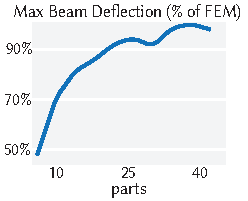
\includegraphics{figures/deflection.pdf}
%	\caption{\revise{Te maximum beam deflection, as a percentage of the FEM beam's maximum deflection, is shown to converge to the FEM result as we add more parts along the beam.}}
%	  \label{fig:plot_beam_deflection}
%\end{wrapfigure}
\begin{figure}[h]
  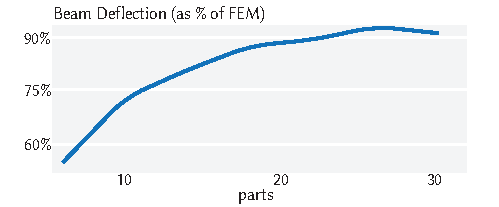
\includegraphics[width=\columnwidth]{figures/deflection_full.pdf}
	\caption{\revise{Te maximum beam deflection, as a percentage of the FEM beam's maximum deflection, is shown to converge to the FEM result as we subdivide the beam.\ty{currently a very blank figure, which I dont mind, but could consider adding inset beam pictures to give an idea of how this experiment works}}}
  \label{fig:plot_beam_deflection}
\end{figure}

We use SEM with quadratic polynomials for this test and observe that our SEM simulation, made of \revise{26} independent NURBS patches, shows good agreement with FEM. Each subdivision of the NURBS beam enables more complicated kinematics, 
but very few surface elements are needed to produce compelling results.


\begin{figure}[h]
  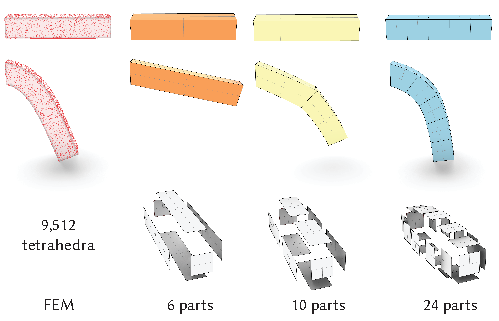
\includegraphics[width=\columnwidth]{figures/beams.pdf}
  \caption{Our SEM simulation is able to qualitatively converge to a high resolution FEM simulation result (left) as we increase the number of surfaces in the model (right). }
  \label{fig:convergence}
\end{figure}

\revise{Additionally, we perform a twisting beam experiment on a 22 part beam model. Despite the relatively small number of NURBS patches, we see in \reffig{beam_twist} that the quadratic polynonmials permit complex deformation.}


\begin{figure}[h]
  \includegraphics[width=\columnwidth]{figures/beam_twist.pdf}
  \caption{\revise{With the left end of the beam held fixed, we show the result of rotating the right end of a 22 part beam up to 360 degrees.}}
  \label{fig:beam_twist}
\end{figure}


\revise{\reffig{scalability} shows a scalability study in which a  unit cube, composed of 6 parts, is extended by appending 4 more parts at a time.
Note that our algorithm scales similarly to standard high-order finite element approaches due to the compact support of our weight functions.}

\begin{figure}[h]
  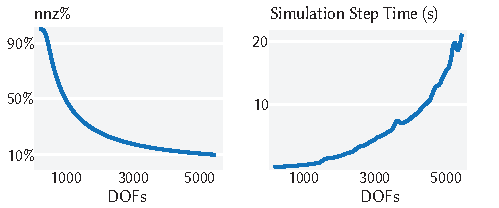
\includegraphics[width=\columnwidth]{figures/scalability.pdf}
  \caption{\revise{Here we progressively add more degrees of freedom to a beam by iteratively inserting 4 part sections, extending the beam in the $x$-axis direction at each step. On the left we report the number of non-zeros as a percentage of the total number of elements in the stiffness matrix (nnz$\%$). The right plot shows the average runtime of a simulation step as the number of degrees of freedom increases.}}
  \label{fig:scalability}
\end{figure}

We also show that our raycasting weight computation is able to create shape-aware output. \reffig{independence} and \reffig{octopus} show that manipulating
parts that are nearby but separated will behave in an appropriately independent fashion. Our grumpy model is capable of extending 
its leg without causing unrealistic deformations in the plant foot, and our octopus model shows independent motion of all eight limbs upon contact with the ground.


\begin{figure}[h]
  \includegraphics[width=\columnwidth]{figures/independent_movement}
  \caption{Our raycasting weight computation produces shape-aware blending weights. Here the locality of our blending weights allows the two legs of the grumpy model to move independently. }
  \label{fig:independence}
\end{figure}

\begin{figure}[h]
  \includegraphics[width=\columnwidth]{figures/octopus.pdf}
  \caption{\revise{We simulate a falling octopus, and observe the 8 limbs moving independently. Self-collision is not accounted for here.}}
  \label{fig:octopus}
\end{figure}

% relaxed modelling constraints
By virtue of its meshless nature, SEM is robust to a wide range of challenging models with large gaps and disconnected primitives.
\reffig{chicken} shows frames from a simulation of a rubber chicken. Note that the chicken model itself features large gaps between the individual NURBS parts. 
Despite the lack of explicit connectivity, the SEM blending weights have the effect of implicitly enforcing connectivity at these seams. 

\begin{figure*}[htp]
  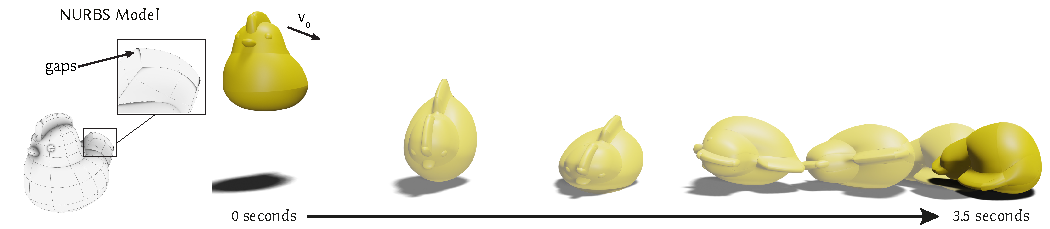
\includegraphics[width=\textwidth]{figures/chicken.pdf}
  \caption{Simulation of a chicken model with gaps between surfaces.}
  \label{fig:chicken}
\end{figure*}

SEM is also robust to intersections in modelling input. \reffig{badmodels} shows simulations of two jelly coffee mugs. 
The top row shows a model with negligible overlap, whereas the bottom row shows the result of a careless modeller who has deeply embedded the handle of the mug in the body in order to attach it, creating a large area of overlap.
In both cases SEM produces a plausible physically-based animation without requiring additional model clean-up.

\begin{figure}[h]
  \includegraphics[width=\columnwidth]{figures/mug_overlap}
  \caption{Our SEM is robust to overlapping regions and self-intersections. Here the simulation result of the coffee mug with overlapping handle (bottom) still matches its corresponding counterpart without negligible overlaps (top). }
  % \caption{Coffee mug with overlapping handle. (top) row of models with increasing overlap (middle) single weight image showing behaviour in the overlapping region, (bottom) simulation result for each one}
  \label{fig:badmodels}
\end{figure}

%different material parameters / material models 
Since the equations of motion for SEM are derived using a general elastic potential, it is theoretically capable of supporting arbitrary elastic constitutive models.
% We derive the equations of motion for SEM using a general elastic potential and thus SEM supports arbitrary constitutive models. 
\reffig{rocket} shows a rocket ship simulated with both high stiffness (steel) and low stiffness materials (rubber). 
In both cases intuitive and visually pleasing results are created wherein the trajectories correctly reflect the desired material characteristics.  
%multiple materials
\begin{figure*}[htp]
  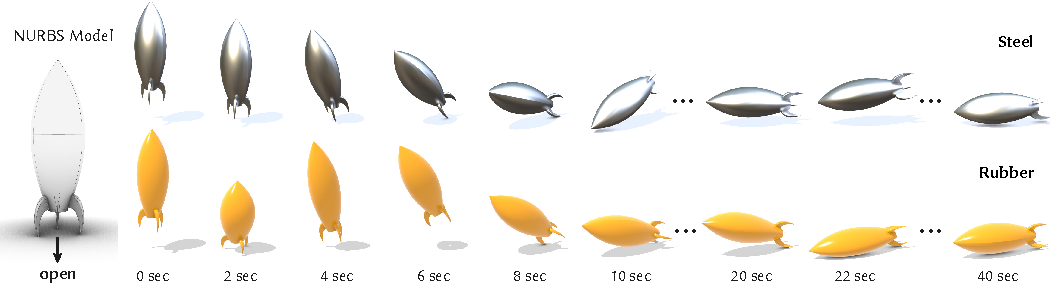
\includegraphics[width=\textwidth]{figures/rocket.pdf}
  \caption{SEM is able to produce animation using a wide variety of material parameters. Here we simulate both a steel and rubber rocket ship. 
  To make this even more challenging, the rocket model is an open surface (at the bottom), but a plausible animation is still generated.}
  \label{fig:rocket}
\end{figure*}

SEM also supports the simulation of objects made up of heterogenous materials. By specifying different material properties inside nested 
parts we are able to simulate a drag racing wheel with a metal hub and soft rubber tread~(\reffig{tire}).

\begin{figure}[h]
  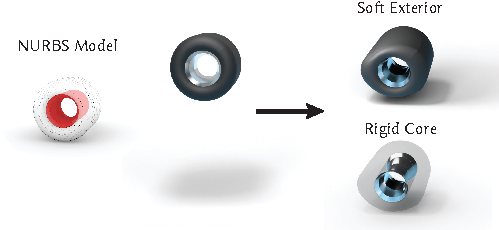
\includegraphics[width=\columnwidth]{figures/tire}
  \caption{Our SEM is directly applicable to the simulation of objects with heterogenous materials.}
  \label{fig:tire}
\end{figure}


% %different surface reps
% Though we focus on NURBS surface representations, the only NURBS specific construction in the SEM method is the Jacobian \refeq{velocity_jacobian}.
% Many other boundary representations admit a linear representation and are thus directly consumable by our method.
% \reffig{subd} shows an example of applying our SEM method to a subdivision model by making such a modification.
% \begin{figure}[h]
%   \includegraphics[width=\columnwidth]{example-image-a}
%   \caption{show subd simulation if we have it. If it works really well we'll just mix subds and nurbs throughout the paper. }
%   \label{fig:subd}
% \end{figure}

% different time integration scheme
\nicetohave{Integration Figure}
%\begin{figure}[h]
%  \includegraphics[width=\columnwidth]{example-image-a}
%  \caption{show mug simulation using newton's method, linearly implicit Euler \Honglin{Maybe I can do that quickly}. }
%  \label{fig:time_integration}
%\end{figure}

%editing example
For downstream applications, the output of  SEM simulation is itself editable in a NURBS modelling program (see \reffig{edit}). 
This can be useful for visual effects pipelines, allowing artists to easily post process animations using the same tools in which they were created.
\begin{figure}[h]
  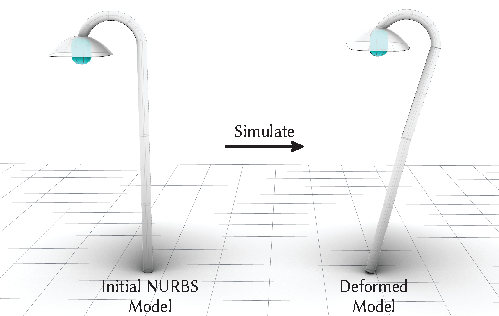
\includegraphics[width=\columnwidth]{figures/export_iges.pdf}
  \caption{Here we show the output of an SEM animation loaded into Rhinoceros 3D 7 for additional editing.\ty{note: initial version of figure. Currently remaking it :)}}
  \label{fig:edit}
\end{figure}

%show stoppers
Finally we show a few additional examples, highlighting the ability of SEM to handle complex simulations involving deformation, contact and friction.
In \reffig{staypuft} we show two astronauts in jaunty space suits collide in zero gravity. 
SEM gracefully allows bounded discontinuities in simulation output to allow for rich motion. 
This is similar to Discontinous Galerkin approaches but in SEM this behavior emerges from the kinematic model, rather than from additional flux terms~\cite{kaufmann2009flexible}.
\revise{Our soft enforcement of part connectivity at boundaries is a result of the weighting function attributing equal weight values to equidistant parts. This equal weighting induces elastic forces that attempt to enforce continuity. In our examples, these discontinuities only introduce minor artifacts affecting the rendering, but this may be addressed using a separate render mesh or by using a representation with explicit connectivity.}

In \reffig{teaser} we directly simulate the NURBS surface model of a bouncy castle under a periodic wind force. 
In \reffig{starship} we show an animation of the Space-V starship landing on Mars in a graceful way. 
This example shows the benefit of NURBS modeling, a relatively small number of primitives can represent a complex shape.
SEM successfully handles the stiff materials, complicated geometry and non-trivial collisions in this scene.

\begin{figure*}[htp]
  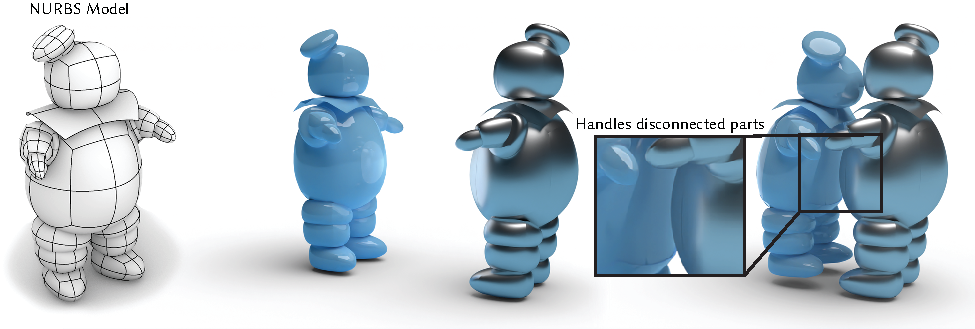
\includegraphics[width=\textwidth]{figures/astronauts.pdf}
  \caption{Two astronauts, in jaunty spacesuits collide while spacewalking in zero-g. SEM correctly handles severely disconnected parts by correctly estimating elastic energy even in discontinuous regions.}
  \label{fig:staypuft}
\end{figure*}

\begin{figure*}[htp]
  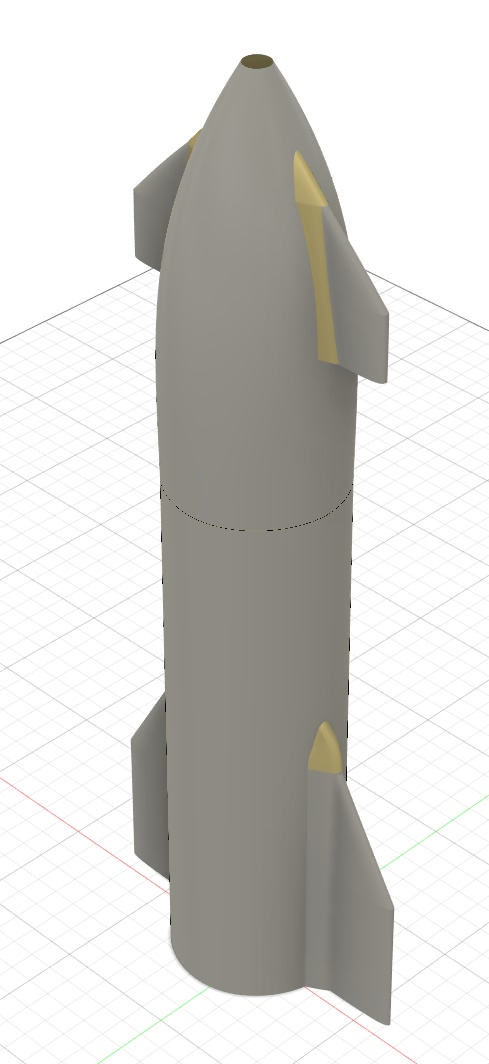
\includegraphics[width=\textwidth,height=3in]{figures/starship.pdf}
  \caption{Our SEM is robust to stiff materials, complicated geometry and non-trivial collisions. Here we show the Space-V starship makes a graceful landing on the rugged surface of Mars. }
  \label{fig:starship}
\end{figure*}
